\chapter{Introduction}
\emph{“ Can physics be simulated by a universal computer? [...] the physical world is quantum mechanical, and therefore the proper problem is the simulation of quantum physics [...] the full description of quantum mechanics for a large a system with R particles [...] has too many variables, it cannot be simulated with a normal computer with a number of elements proportional to R [ ... but it can be simulated with ] quantum computer elements. [...] Can a quantum system be probabilistically simulated by a classical (probabilistic, I’d assume) universal computer? [...] If you take the computer to be the classical kind I’ve described so far [..] the answer is certainly, No! “} 
\begin{flushright}
Richard P Feynman \cite{feynman82}\cite{nielsen}
\end{flushright}


The primary aim of any sort of simulation is to solve the differential equation that governs the dynamics of the system. One of the most simple example one can provide of such an equation is the Newtons equation of motion,
\begin{equation}
m\frac{d^{2}x}{dx} = F
\end{equation}
Generally, the initial state of the system would be input to the problem. Using simulations one aims to predict the state of the system at a later time or position. The first step in doing any sort of simulation is encoding the state of the system digitally, which more often involves some approximation. Using the encoding we have to prepare the initial state of the system. Then one has to discretize the dynamical differential equation in space and time. Discretization should be done in such a way that the iterative application of a procedure should evolve the state from initial to final conditions. The accuracy of the output state predicted by the simulator depends upon discretization. Theoretically, as the length of discretization decreases the result would be more accurate. But while computing we need to take into consideration of other sorts of errors that can happen while decreasing the discretization length and often have to find an optimum value. Why this approach works?. This works because the error in is such an approach is bounded and not considerably grows as the number of iterations increases\cite{nielsen}. Further, only those system that can be efficiently described can be simulated efficiently. Thus there are systems where such an approach fails.

When it comes to the question of whether we can simulate a quantum system using a classical simulator, the short answer is yes. But it should be noted that often such simulations are inefficient and fail when the number of particles in the system is very high.  When we analyse the problem of simulating a quantum system, for most of the simple quantum systems, the evolution is given by the time-independent Schrodinger equation. 
\begin{equation}
i\hbar \frac{d}{dt}\ket{\psi} = H \ket{\psi}
\end{equation}
On the position basis, the above equation will be 
\begin{equation}
i\hbar\frac{\partial}{\partial t}\psi(x)= [-\frac{\partial^{2}}{\partial x^{2}}+V(x)]\psi(x)
\end{equation}
Where $\braket{x|\psi} = \psi(x)$.
Assume that we wish to simulate a simple two-level system ( Qubit ) that obeys the above time-independent Schrodinger equation. For a single qubit system, we have to solve two differential equation, for a two-qubit system it would be four equations and so on. Thus, a general system of n qubits $2^{n}$ differential equations must be solved to simulate it. This exponential explosion in the equation is unavoidable unless we employ some approximate methods like Monte Carlo methods\cite{monte} which considerably reduce the number of equations. Such classical stochastic methods would allow us to evaluate the phase-space integrals of many-body quantum systems in polynomial time. But these methods are efficient while the function being integrated does not change its sign. Thus while using such methods sampling of the function is done in a relatively small number of points. For systems like fermionic or frustrated systems, the integrals encounter the problem of sampling with non-positive semi-definite functions (referred to as negative sign problem\cite{troyer} \cite{georgescu} ) which cause an exponential increase in computation time as the number of particles increases. Thus in such systems, Monte Carlo methods are shown to be inefficient. Other than Monte Carlo methods there are methods like Density Functional Theory (DFT) \cite{dft}, mean-field theories, Green function-based methods, many-body perturbation theories \cite{mbpt} etc. which also have similar issues that restrict its application to some particular types of quantum systems.

Richard P Feynman was one of the persons who put forward a solution to this problem. He said that \emph{“ Let the computer itself be built of quantum mechanical elements which obeys quantum mechanical laws “} \cite{feynman82}. Feynman realized that such a quantum system - which later called a quantum computer - would be able to handle the exponential explosion of parameters that happen while solving a large number of equations without using an exponentially large number of physical resources. Even though Feynman proposed such a radical idea, he was not aware of how to realise simulations in such controllable quantum systems. More than a decade later, It was Lloyd who showed that quantum computer could act as a universal quantum computer \cite{lloyd}. Here the term “universal” is used in the sense that the same system can be used to simulate vastly different problems. Of course, one has to make adjustments in the programs for tackling different problems. 

Even though the quantum computer was proposed to simulate quantum mechanics, its uses extend far beyond it. The past three decades have revealed the true power of a quantum computer. Nowadays quantum computing and quantum information itself a topic of research. Further, it became later clear that we don’t always need a quantum computer for implementing quantum simulations. For simulating a particular quantum system, we only need a simpler quantum system that has similar time evolution. That is, simpler quantum devices that mimic the time evolution of other quantum systems can be used as simulators. But the drawback of such an approach is that such a simulator would be problem-specific ( not universal ). On the bright side, such simple systems can be easily controlled and designed compared to sophisticated quantum computers.

Based on the approach, we can broadly classify the quantum simulations into kinds; Analog Quantum Simulation (AQS) and Digital Quantum Simulations (DQS). In DQS we use quantum computers as simulators. Here we encode the time evolution of the quantum system in a quantum circuit comprising qubits and quantum gates.  The circuit is designed in such a way that the output of the circuit gives the time evolved state of the system under study.  A similar but different approach is taken in Analog Quantum Simulations. In AQS, a simple quantum system that is controllable is created depending upon the problem. This system is designed in such a way that it would mimic the time evolution of the system under study. Thus in this approach, simulations are done using a simple system as simulators.

In recent years, the field of quantum simulations has gained momentum. The sudden spike in interest is two folds. The first one is its wide range of application. For instance, quantum simulations can be used in condensed matter for studying many difficult problems like quantum phase transitions, high Tc superconductivity, quantum magnetism etc. Other potential applications include fields like high energy physics, nuclear physics, cosmology, quantum chemistry etc. The second factor that accelerated the growth of quantum simulations is the recent progress in the field of quantum technologies. Recent years have witnessed development in different types of realization of quantum computers. Nowadays quantum computers are publicly accessible. Quantum simulators now available can be used to repeat the simulations many times. Technologies to maintain coherent control over the system and to perform non-demolition projective measurement have matured enough to make it possible.

In near future, quantum simulations will become a prominent tool for research for a wide variety of fields. In this milieu, the study of quantum simulations holds importance. This was the motivation for us to conduct this study. Here we are interested in the digital quantum simulations of phenomena called Neutrino oscillation. We use the quantum computing services provided online to carry out our simulations. The scheme for such a simulation was put forward by Arg\"ulles and jones in 2017 \cite{jones}. They have encoded neutrino oscillation into a quantum circuit. Time evolution of the qubits is done by applying unitary single and two-qubit gates. The exact scheme will be discussed in the following sections. 

In nature, neutrinos are produced in three distinct flavours electron, muon and tau. Neutrinos are produced through weak interactions. As neutrino beam propagates from source to detector neutrino flavour oscillate between the three flavours. The first evidence of neutrino exhibit flavour oscillation from the famous Ray Davis Homestake experiment \cite{ray}.  He reported a deficit in the flux of solar neutrinos (electron neutrinos)  from the value predicted by the Standard model. He used a chlorine-based detector and obtained a flux that was three times less than that of the theoretical value.  This observation of Ray Davis later came to be known “Solar Neutrino Problem”. For the contributions in the field of astrophysics, Ray Davis was awarded the Nobel prize in Physics in 2002. 

Following the Homestake experiment, different sort of powerful detectors was set up and studied the problem. All the experiments confirmed the deficit of neutrinos in the solar flux. Ray Davis performed his experiment in the 1960s. Interestingly, the idea of neutrino oscillation was put forward by Pontecorvo in 1957\cite{ponte57}. Thus one can say that solution existed even before the problem. But in Pontecorvo’s version neutrino-anti neutrino undergo oscillation. He put forward this theory in analogy with the neutral kaon mixing that was known way before. Although such oscillations do not occur in nature, this formed a key conceptual foundation in developing the theory for neutrino oscillation. The theory for neutrino flavour oscillation was put forward first by Maki, Nakagawa, Sakata in 1962 which was later elaborated by Pontecorvo in 1967 \cite{ponte68}. The solar neutrino deficit observed only a year after that. The solar neutrino problem baffled scientists for a long time. It was the team of Canadian scientists lead by Arthur B McDonald in Sudurbary Neutrino Observatory (SNO) that put an end to the mystery. They experimentally verified that electron neutrino produced in the sun undergo flavour oscillations. The deficit in the number of electron neutrinos was because neutrinos undergo flavour change while travelling to Earth\cite{mcdonald}. At the same time, a group of Japanese scientist lead by Takaaki Kajita verified neutrino oscillation by studying atmospheric neutrinos. Atmospheric neutrinos were produced when cosmic rays hit the Earth’s atmosphere. When it travels to the Earths surface they undergo flavour oscillations. The team led by Kajita was able to detect these flavour oscillations. For the experimental verification of neutrino flavour oscillation, both Kajita and McDonald was awarded the Nobel prize in physics in 2015.

The verification that neutrinos can undergo oscillations comes with great consequences. It was known that neutrinos can undergo flavour oscillation only if they have mass. But according to the Standard Model, neutrinos are massless. Thus the phenomenon of neutrino oscillation insists on the modification of the standard model. From neutrino oscillation measurement one can find out mass squared splittings and mixing angles ( will discuss it later ). But till now the actual mass of the three neutrinos are still unknown. Even though there are some minimal extensions of the Standard model to accomodate neutrino masses, exact theory is unknown. Thus the study of neutrino oscillation is a door to explore physics outside the standard model.


A typical Neutrino flavour change is depicted in the figure $\ref*{fig 1}$. A neutrino source produces a neutrino along with charged lepton.Flavour of the lepton ($e,\mu$,or $\tau$) produced would give us the flavour of neutrino produced ($\nu_{e},\nu_{\mu}$,or $\nu_{\tau}$). A neutrino created in a specific flavour eigenstate would be in coherent superposition of all three mass eigenstates. This is coherent superposition impies that we cannot experimentally find out which mass state is produced at the interaction vertex of feynman diagram. But the proportion of each mass state in the produced pure flavour state has been found to depend profoundly on that flavour. The relationship between flavour and mass states is encoded in the PMNS (Pontecorvo Maki Nakagawa Sakata) matrix. It is a unitary mixing matrix that contains information on the mismatch of quantum states of neutrinos when they propagate freely and when they take part in the weak interactions. Experiments have established values for the elements of this matrix \cite{zyla}.\par
\begin{figure}[h]
\graphicspath{ {./Images/} }	
{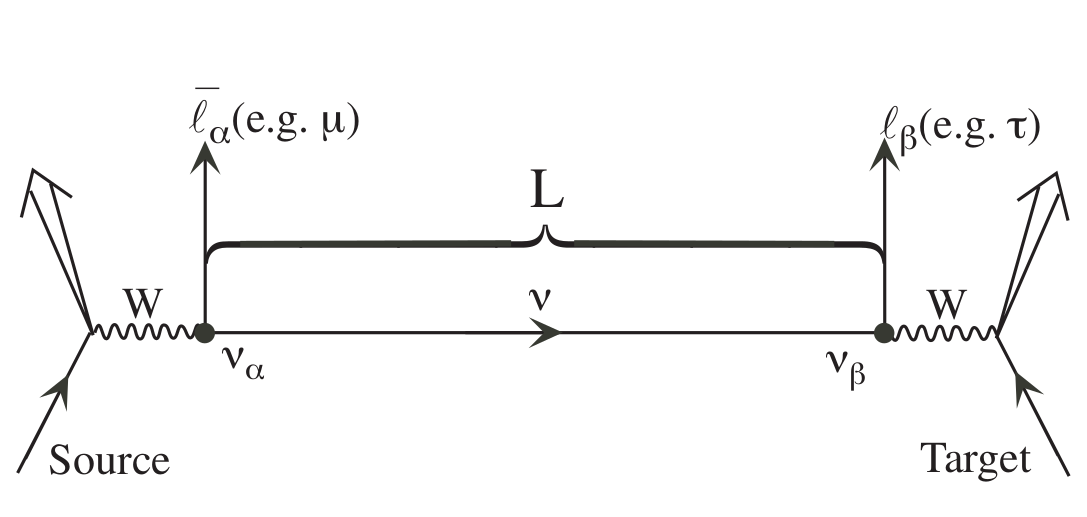
\includegraphics[width=\textwidth]{fig_1.png}}
\centering

\caption{ Neutrino flavour change in vaccum\cite{kayser}.}
\label{fig 1}
\end{figure}


Experimentally a neutrino beam of known flux and flavour $\alpha$ is produced and send to a detector placed at a distance $L$ from the source. There it would interact with the detector material to produce a secondary lepton, let say $l_{\beta}$.  Thus at the time of interaction(with detector material), the neutrino would in $\beta$ flavour state ( $\nu_{\beta}$ ). One could detect the flavour change in two ways. One way is observe the appearance of neutrinos of new flavour $\beta$ that is different from the original flavour ( $\beta\neq\alpha$). Such type of experiments are called appearance experiments and would give appearance probability. The other way to is to observe thatsome of this known flavour $\nu_{\alpha}$ disappears. Such type of experiments are called disappearance experiments and would give disappearance probability or survival probability.
